\documentclass[xcolor={pdftex,dvipsnames,table}]{beamer}

\usepackage[english]{babel}
\usepackage{tikz,comment,amssymb}
\usetikzlibrary{shapes}
\usetikzlibrary{arrows}
\usetikzlibrary{mindmap}
\usetikzlibrary{trees}
\usepackage{bm}
\usepackage{fancyvrb}
\usepackage{arydshln}
\usetikzlibrary{patterns}
\usepackage[normalem]{ulem}
\usepackage{fancybox}
\usepackage{hyperref}

\definecolor{redUnipd}{HTML}{9b0014}
\definecolor{grayUnipd}{HTML}{444F51}
\definecolor{myblue}{HTML}{317a9b}
\definecolor{gray64}{RGB}{0,62,114}
\usefonttheme{structurebold}
\usecolortheme[named=myblue]{structure}
\setbeamercolor{palette primary}{fg=myblue,bg=white} 
\setbeamercolor{palette secondary}{bg=myblue,fg=white}
\setbeamercolor{palette tertiary}{bg=white,fg=myblue}
\setbeamercolor{palette quaternary}{bg=white,fg=myblue}
\setbeamerfont{frametitle}{size=\LARGE}

\useinnertheme{circles}
%\useoutertheme[subsection=false]{smoothbars}
\setbeamerfont{frametitle}{series=\bfseries}
\usepackage{cmbright}

\newcommand{\bb}[1]{\begin{block}{#1}}
\newcommand{\eb}{\end{block}}
\newcommand{\bi}{\begin {itemize}}
\newcommand{\ei}{\end{itemize}}
\newcommand{\be}{\begin {enumerate}}
\newcommand{\ee}{\end{enumerate}}
\newcommand{\bfr}[1]{\begin{frame} \frametitle{#1}}
\newcommand{\mytilde}{$\sim$}
\newcommand{\Perm}{\Pi}
\newcommand{\HH}{\mathbf{H}}
\newcommand{\IH}{(\mathbf{I}_n-\mathbf{H})}


\AtBeginSection[] {
  \begin{frame}<beamer>
    \frametitle{Outline}
    \tableofcontents[currentsection]
 \end{frame}
}


\title{Multivariate Permutation tests in presence of nuisances (i.e. Covariates)}
\author{Livio Finos}
\institute{University of Padova}
\logo{\includegraphics[scale=.1]{figures_perm_covariates/logoUnipd.jpg}}
\date{}
\begin{document}

%% ==========================TITLE PAGE
{
\begin{frame}
\titlepage
\end{frame}
}
%% ==========================OUTLINE
%\begin{frame}<beamer>
%  \frametitle{Outline}
%\tableofcontents
%\end{frame}

\begin{frame}
\frametitle{(minimal) Bibliography}

\begin{itemize}
\item Anderson M. Winkler, Gerard R. Ridgway, Matthew A. Webster, Stephen M. Smith, Thomas E. Nichols (2014)
Permutation inference for the general linear model.
NeuroImage, 92, \url{doi.org/10.1016/j.neuroimage.2014.01.060}
\item Sara Kherad-Pajouh, Olivier Renaud (2010) An exact permutation method for testing any effect in balanced and unbalanced fixed effect ANOVA. Computational Statistics and Data Analysis. \url{doi:10.1016/j.csda.2010.02.015}
%\item Sara Kherad-Pajouh, Olivier Renaud (2015) A general permutation approach for analyzing repeated measures ANOVA and mixed-model designs. Stat Papers \url{doi:10.1007/s00362-014-0617-3}
\item Aldo Solari, Livio Finos and Jelle Goeman (2014) Rotation-based multiple testing in the multivariate linear model.
Biometrics, 70, \url{doi.org/10.1111/biom.12238}
\end{itemize}

\end{frame}

%%% ==========================INTRO

\begin{frame}[fragile]
\frametitle{Motivating example}
\bi
\item Acute Lymphoblastic Leukemia data (Chiaretti et al., 2004)
\item $n =$ 128 patients
\item $p =$ 12625 gene expression profiles
\item covariate of interest: \verb"group" (B or T-cell type patients)
%\item confounder(s): \verb"age" (+ \verb"sex", \verb"mdr", \verb"stage", \verb"kinet")
\item differentially expressed genes between the two groups?
\ei
\small
\[
\verb"gene" \,\, = \,\, \gamma_0 \,\,+ \,\, \textcolor{myblue}{\beta}  \cdot {\tt group}  \,\, + \,\,  \verb"error" 
\]

\pause

 \[
\left[\begin{array}{c}
    \verb"gene"_1 \\ 
    \vdots \\
    \verb"gene"_p \\ 
  \end{array}\right] = 
  \left[\begin{array}{c}
    \gamma_{01} \\ 
        \vdots \\
    \gamma_{0p} \\ 
  \end{array}\right] + \,\,  \left[\begin{array}{c}
    \textcolor{myblue}{\beta_{1}} \\ 
        \vdots \\
    \textcolor{myblue}{\beta_{p}} \\ 
  \end{array}\right] \, \cdot \, \verb"group" \,\, +  \,\, \left[\begin{array}{c}
    \verb"error"_1 \\ 
        \vdots \\
    \verb"error"_p \\ 
  \end{array}\right]
 \] 


\end{frame}
%%======================
\begin{frame}[fragile]
\frametitle{Multivariate linear model}

\begin{eqnarray*}
\mathbf{Y} = \mathbf{1}\mathbf{G}_{1\times p} +  \mathbf{X}\mathbf{B}_{1\times p} + \mathbf{E}
\end{eqnarray*}
\bi
\item $\mathbf{Y}$ : $( n \times p)$ matrix of responses
\item $\mathbf{X}$ : $( n \times 1)$ matrix of covariates ({\tt group})
\item $\mathbf{E} \sim (\mathbf{0}_{n\times p}, \mathbf{I}_{n} \otimes \mathbf{\Sigma} )$ matrix of errors
\item[] $\ \ \ \ \mathbf{\Sigma}$ : $(p \times p)$ gene-gene covariance matrix
\ei 


\bb{Marginal model ($j$-th gene)}
\[
\bm{y}_{j}=  \mathbf{1}  \bm{\gamma}_{0j} + \mathbf{X} \bm{\beta}_{j} +\bm{\varepsilon}_{j}, \qquad  \bm{\varepsilon}_{j}\sim (\mathbf{0}_{n\times 1}, \sigma_j^2 \mathbf{I}_{n}  )
\]
\eb
\bb{Multiple hypotheses}
\[
H_j :  \bm{\beta}_{j} = \bm{0},\ \textcolor{redUnipd}{\forall \bm{\gamma}_{j}} \qquad j=1,\ldots,p
\]
\eb

\end{frame}
%===============
\begin{frame}[fragile]
\frametitle{The Multiple Testing Problem}
 \[
\left[\begin{array}{c}
    \verb"gene"_1 \\ 
    \vdots \\
    \verb"gene"_p \\ 
  \end{array}\right] = 
  \left[\begin{array}{c}
    \gamma_{01} \\ 
        \vdots \\
    \gamma_{0p} \\ 
  \end{array}\right] + \,\,  \left[\begin{array}{c}
    \textcolor{myblue}{\beta_{1}} \\ 
        \vdots \\
    \textcolor{myblue}{\beta_{p}} \\ 
  \end{array}\right] \, \cdot \, \verb"group" \,\, +  \,\, \left[\begin{array}{c}
    \verb"error"_1 \\ 
        \vdots \\
    \verb"error"_p \\ 
  \end{array}\right]
 \] 
\pause
$H_{0j}:\beta_{j}=0\ (=\textrm{two grous are equal})\ \,\ j=1,\ldots,p$\\
\bigskip
\pause
$\ \ \ \ \ \ \ $ one p-value for each gene ($p$)
\end{frame}

% \begin{frame}
% \frametitle{a problem of Multiplicity}
% Remark: Probability of Type I error: $P(p-value<0.05 |H_0)=0.05=1/20$\\
% \bigskip
% \pause
% Analogy with 20-sided dice: 
% 
% %\begin{eqnarray*}
% \begin{tabular}{l}
% P( \includegraphics[scale=.1]{figures_perm_covariates/20diceB.jpg} )=1/20=.05
% \end{tabular}
% %\end{eqnarray*}
% \bigskip
% \pause
% 
% and what if we have many dices?
% \pause
% 
% \begin{eqnarray*}
% P(\textcolor{myblue}{At\ least\ 1}\includegraphics[scale=.1]{figures_perm_covariates/20diceB.jpg} \includegraphics[scale=.1]{figures_perm_covariates/20diceB.jpg} \includegraphics[scale=.1]{figures_perm_covariates/20diceB.jpg} \includegraphics[scale=.1]{figures_perm_covariates/20diceB.jpg}\includegraphics[scale=.1]{figures_perm_covariates/20diceB.jpg})=?\pause = 1-(1-1/20)^5= \textcolor{myblue}{.226}
% \end{eqnarray*}
% 
% \pause
% and
% \begin{eqnarray*}
% P\big(\textcolor{myblue}{At\ least\ 1} \includegraphics[scale=.1]{figures_perm_covariates/20diceB.jpg} \includegraphics[scale=.1]{figures_perm_covariates/20diceB.jpg} \includegraphics[scale=.1]{figures_perm_covariates/20diceB.jpg} \includegraphics[scale=.1]{figures_perm_covariates/20diceB.jpg}\includegraphics[scale=.1]{figures_perm_covariates/20diceB.jpg}
% \includegraphics[scale=.1]{figures_perm_covariates/20diceB.jpg} \includegraphics[scale=.1]{figures_perm_covariates/20diceB.jpg} \includegraphics[scale=.1]{figures_perm_covariates/20diceB.jpg} \includegraphics[scale=.1]{figures_perm_covariates/20diceB.jpg}\includegraphics[scale=.1]{figures_perm_covariates/20diceB.jpg})=?\pause \\ = 1-(1-1/20)^{10}= 
% \textcolor{myblue}{.401}
% \end{eqnarray*}
% 
% 
% \end{frame}


\begin{frame}
\frametitle{Type I error if not correcting \\ for multiple testing}%
\begin{center}
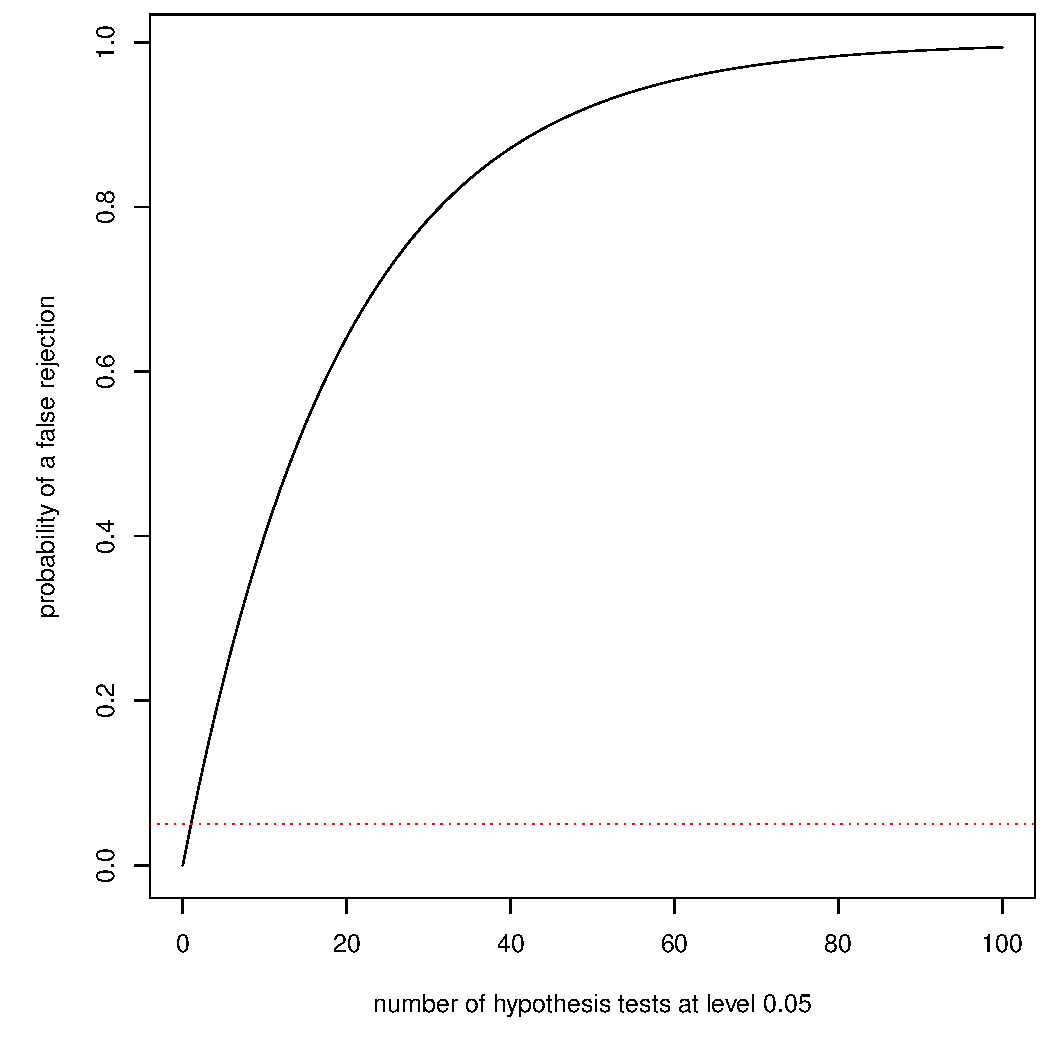
\includegraphics[height=7cm]{figures_perm_covariates/typeI}
\end{center}
\end{frame}



\begin{frame}
\frametitle{\ldots a very common problem}

The problem of multiplicity control arises when more than one (statistical) hypothesis is tested \\(12625 in this case, one for each gene).\\
\bigskip
This problem is very common in many (other) fields of medicine:
\begin{itemize}
\item[$\circ$] clinical trials with multiple endpoints
\item[$\circ$] neuroimaging experiments
\end{itemize}
and in many other fields like:
\begin{itemize}
\item[$\circ$] psycho-sociological
\item[$\circ$] ecological
\item[$\circ$] quality control
\item[$\circ$] many others...
\end{itemize}

\end{frame}
%==================
%\begin{frame}
%\frametitle{The Error Measures in a Multivariate Framework}
%{\bf A Toy example:} 10 000 hypotheses are tested at level $\alpha=0.05$.\\ 
%ALL of them are under $H_0$, the test statistics are independent. 
%\begin{itemize}
%\item[$-$] $P(\textrm{reject hypothesis } i)=P(\textrm{Type I error in test } i)\leq .05$\\  $\forall\ i=1,\ldots,10 000$ \pause
%\item[$-$] 500 wrong rejections (i.e. type I errors) hypotheses on average
%\item[$-$]$P(\textrm{at least 1 type I error}) \cong 1$
%\end{itemize}
%\bigskip 
%\pause
%Of course in real data usually: 
%\begin{itemize}
%\item[$.$] NOT all Null Hypotheses ($H_0$)
%\item[$.$] Original variables (i.e. derived tests) are dependent  \pause
%\item[]  even more fun!
%\end{itemize}
%\end{frame}


%\begin{frame}
%\frametitle{Choose the Error Measures to control}
%\begin{itemize}
%\item[$\circ$]{\bf FamilyWise Error Rate (FWER)} \\
%$\ \ \ $P(wrong rejections $\geq 1$)
%\item[$\circ$]{\bf Generalized FamilyWise Error Rate ($k$-FWER)}\\ (Lehmann and Romano, 2005)\\
%$\ \ \ $ P(wrong rejections $\geq k$)
%\item[$\circ$]{\bf False discovery Exceedance (FDX)}\\ (Genovese and Wasserman, 2004)\\
%$\ \ \ $ P(wrong / all rejections $\geq q$)
%\item[$\circ$]{\bf False discovery Rate (FDR)} \\ (Benjamini and Hochberg, 1995)\\
%$\ \ \ $ E(wrong / all rejections )
%\end{itemize}
%\bigskip

%\end{frame}

\begin{frame}
\frametitle{Familywise Error Rate (FWER)}
\textcolor{myblue}{FWER: \\ probability of one or more false positives (i.e. wrong rejections)} 

%$$\textrm{FWER}=P( At\ least\ 1\ false\ positive)$$
%control of the FWER (at joint level $\alpha$) requires that $FWER \leq \alpha$.

\bb{}
The most well-known method controlling the FWER: \\
 \textcolor{myblue}{Holm} procedure (Holm, 1979). \\
Based on step-wise application of Bonferroni inequality:\\
hence: reject genes with $p_{i}\leq \alpha/(\textrm{\# of genes}),\ i=1,\ldots,12625$\\
\pause
Is valid for every form of \textcolor{myblue}{dependence} among p-values. \\
\pause
BUT becomes \textcolor{myblue}{very conservative} when dependencies are strong.\\
\pause
Permutation tests are often a solution.
\eb
\end{frame}
%% ==========================
%%% ==========================
%%% ========================== Joint distribution
\section{Dealing with dependence among tests}
%%% ========================== Multiplicity Control
\begin{frame}
\frametitle{(Multivariate) Permutation tests}
Under $H_0: \bigcap_{j=1}^{p}H_{j}$,% (drop the $0$ for simplicity $H: \bigcap_{j=1}^{p}H_{j}$ ),
\[
\mathbf{Y} \stackrel{\mathrm{d}}{=} \Perm\mathbf{Y} 
\]
for every permutation matrix $\Perm$ (\emph{null-invariant transformation})
i.e. \textcolor{redUnipd}{Exchangeability}: $f(\mathbf{Y})=f(\Perm\mathbf{Y})$

\bigskip
\pause
\bb{When it holds}
re-sampling null datasets is possible
\eb


\begin{eqnarray*}
\text{$n$-vector }\mathbf{X}= 
\begin{cases}
-1/n_B & \text{ if B patient},\\
+1/n_T & \text{ if T patient}.\\
\end{cases}  
\end{eqnarray*}

(vector of) Test Statistic: 
$t_{obs} = \mathbf{X}^\mathsf{T} \mathbf{Y}$

(vector of) Test Statistic of permuted data: 
$t_{\Perm} = \mathbf{X}^\mathsf{T}  \Perm \mathbf{Y}$

\end{frame}
%%% ==========================
%\begin{frame}
%\frametitle{Exchangeability}
%FORSE VIA
%\bb{No confounders}
%{
%\bi
%\item Null model:
%$
%\displaystyle \mathbf{Y} =  \mathbf{1}_{n\times 1}\mathbf{G}_0 + \mathbf{E}
%$

%\item Independent subjects $\stackrel{\mathrm{i.d.}}{\sim}(\mathbf{G}_0^\mathsf{T},\mathbf{\Sigma})$ 

%\item $\displaystyle  \mathbf{Y} \stackrel{\mathrm{d}}{=} \Perm\mathbf{Y} $ 

%\ei
%}
%\eb

%\end{frame}
%===================
\begin{frame}[fragile]

\frametitle{Joint distributions of P-values }
\bi
\item Observed statistic is any among possible permutations ($\Perm=\mathbb{I}$)
\item compute test statistics on every possible permutation or sample them (e.g. 10 000 random permutations).
\pause 
\item This provides the joint distribution of the test statistics
\pause
\item Compute the joint distribution of p-values from joint dist. of test statistic\\
(compute p-values for observed test stat. and for all permuted test stats.)
\ei

\end{frame}
%%%% ==========================
\begin{frame}
\frametitle{Joint distributions of P-values }
%\frametitle{Rotation null distribution of P-values}

\begin{columns}

 \column{.45\textwidth} 

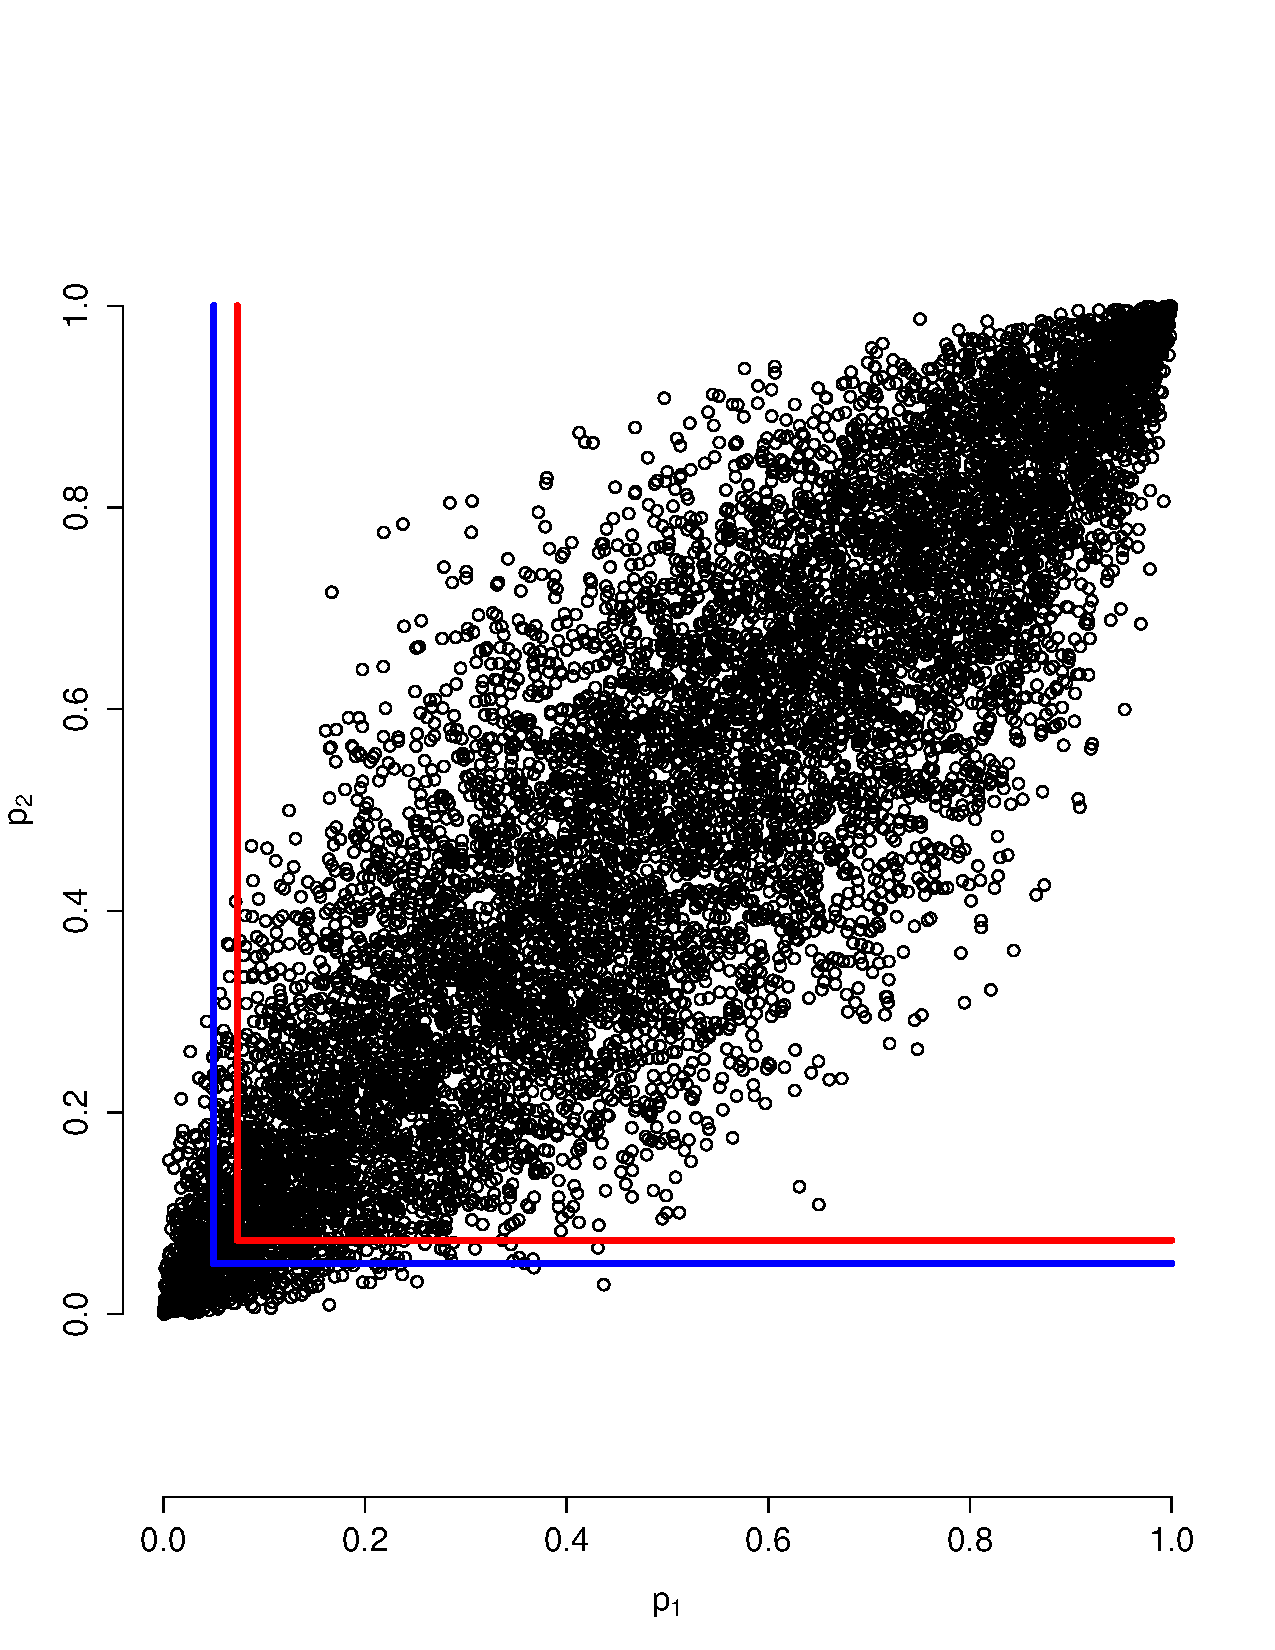
\includegraphics[scale=.28]{figures_perm_covariates/bonferroni}

 \column{.55\textwidth} 


\bi

\item Hypothesis:
\[
H: H_1 \cap H_2
\]

\item \textcolor{red}{min-p} test:
\[
\displaystyle \Pr_H\Big\{\min(p_1,p_2) < c \Big\} \leq \alpha
\]


\item \textcolor{blue}{Bonferroni} inequality:\\

\[c=\alpha/2\]

\ei

\end{columns}

\end{frame}

%%% ========================== Holm vs Westfall & Young min-p
\begin{frame}[fragile]
\frametitle{Holm vs Westfall \& Young min-p}
\pause
Holm: Repeat Bonferroni inequality,\\
\pause
Westfall \& Young: Repeat  min-p step,\\ 
\pause
\bigskip
both provides a list of adjusted p-values

W\&Y is usually more powerful \\ (i.e. lower adjusted p-values, more rejections) than Holm\\
\pause
\medskip
this is because permutation tests account for dependence.\\
\pause
\medskip
You can perform it on {\tt R} using \\ {\tt library(multtest)} or {\tt library(flip)}

\end{frame}
%% ==========================
%%% ==========================
%\begin{frame}
%\frametitle{Sequential}

%\bb{Holm vs Westfall \& Young step-down}
%     \bi
%     \item Start with all hypotheses
%     \item Repeat
%          \bi
%          \item Do Holm/W\&Y to calculate $c$
%          \item Reject hypotheses with $p$-values $< c$
%          \item Remove rejected hypotheses
%          \ei
%     \item Until no new rejection occur
%     \ei
%\eb


%\bb{Improved lower bound}
%\[
%f_{\alpha}(t) \geq \# R_{c^{*}} 
%\]
%where $c^{*}$ is the last critical value obtained
%\eb


%\end{frame}
%%=========================
%\begin{frame}[fragile]
%\frametitle{Goal}

%Multiplicity control:
%\begin{enumerate}

%\bigskip
%\item dealing with dependencies among test statistics\\ (i.e. more powerful methods)

%\bigskip
%\item and adjusting for confounders $ \mathbf{Z}$

%\end{enumerate}


%\end{frame}
%% ==========================
%% ==========================
\section{Confounding}
%% ========================== nuisance factors (i.e. discrete)
\begin{frame}[fragile]
\frametitle{Motivating example}

\bi
\item Acute Lymphoblastic Leukemia data (Chiaretti et al., 2004)
\item $n =$ 128 patients
\item $p =$ 12625 genes
\item covariate of interest: \verb"group" (B or T-cell type patients)
\item \textcolor{redUnipd}{confounder}: \verb"sex"
\item differentially expressed genes between the two groups?
\ei

\small
\[
\verb"gene" \,\, = \,\, \gamma_0 \,\,+ \,\, \textcolor{redUnipd}{\gamma_1} \cdot  {\tt sex}  \,\,  + \,\, \textcolor{myblue}{\beta}  \cdot {\tt group}  \,\, + \,\,  \verb"error" 
\]

 \[
\left[\begin{array}{c}
    \verb"gene"_1 \\ 
    \vdots \\
    \verb"gene"_p \\ 
  \end{array}\right] = 
  \left[\begin{array}{c}
    \gamma_{01} \\ 
        \vdots \\
    \gamma_{0p} \\ 
  \end{array}\right] +   \left[\begin{array}{c}
    \textcolor{redUnipd}{\gamma_{11}} \\ 
    \textcolor{redUnipd}{\vdots} \\
    \textcolor{redUnipd}{\gamma_{1p}} \\ 
  \end{array}\right] \, \cdot \, \verb"sex" \,\, + \,\,  \left[\begin{array}{c}
    \textcolor{myblue}{\beta_{1}} \\ 
    \textcolor{myblue}{\vdots} \\
    \textcolor{myblue}{\beta_{p}} \\ 
  \end{array}\right] \, \cdot \, \verb"group" \,\, +  \,\, \left[\begin{array}{c}
    \verb"error"_1 \\ 
        \vdots \\
    \verb"error"_p \\ 
  \end{array}\right]
 \] 

\end{frame}
%%% ==========================

%\begin{frame}[fragile]
%\frametitle{No confounders (i.e. intercept)}

%\begin{eqnarray*}
%\mathbf{Y} = \mathbf{1}\mathbf{G} +  \mathbf{X}\mathbf{B} + \mathbf{E}
%\end{eqnarray*}
%\bi
%\item $\mathbf{Y}$ : $( n \times p)$ matrix of responses
%\item $\mathbf{X}$ : $( n \times q)$ matrix of covariates ({\tt group})
%\item  $\mathbf{1}$ : $(n \times 1)$ intercept
%\item $\mathbf{E} \sim (\mathbf{0}_{n\times p}, \mathbf{I}_{n} \otimes \mathbf{\Sigma} )$ matrix of errors
%\item[] $\ \ \ \ \mathbf{\Sigma}$ : $(p \times p)$ gene-gene covariance matrix
%\ei 


%\bb{Marginal model ($j$-th gene)}
%\[
%\bm{y}_{j}=  \mathbf{1}  \bm{\gamma}_{j} + \mathbf{X} \bm{\beta}_{j} +\bm{\varepsilon}_{j}, \qquad  \bm{\varepsilon}_{j}\sim (\mathbf{0}_{n\times 1}, \sigma_j^2 \mathbf{I}_{n}  )
%\]
%\eb
%\bb{Multiple hypotheses}
%\[
%H_j :  \bm{\beta}_{j} = \bm{0}, \qquad j=1,\ldots,p
%\]
%\eb

%\end{frame}
%%% ==========================
\begin{frame}[fragile]
\frametitle{Multivariate linear model}

\begin{eqnarray*}
\mathbf{Y} = \mathbf{Z}\mathbf{G} +  \mathbf{X}\mathbf{B} + \mathbf{E}
\end{eqnarray*}
\bi
\item $\mathbf{Y}$ : $( n \times p)$ matrix of responses
\item $\mathbf{X}$ : $( n \times q)$ matrix of covariates ({\tt group})
\item  \textcolor{redUnipd}{$\mathbf{Z}$ : $(n \times 2)$ intercept and {\tt sex}}
\item $\mathbf{E} \sim (\mathbf{0}_{n\times p}, \mathbf{I}_{n} \otimes \mathbf{\Sigma} )$ matrix of errors
\item[] $\ \ \ \ \mathbf{\Sigma}$ : $(p \times p)$ gene-gene covariance matrix
\ei 


\bb{Marginal model ($j$-th gene)}
\[
\bm{y}_{j}=  \mathbf{Z}  \bm{\gamma}_{j} + \mathbf{X} \bm{\beta}_{j} +\bm{\varepsilon}_{j}, \qquad  \bm{\varepsilon}_{j}\sim (\mathbf{0}_{n\times 1}, \sigma_j^2 \mathbf{I}_{n}  )
\]
\eb
\bb{Multiple hypotheses}
\[
H_j :  \bm{\beta}_{j} = \bm{0},\ \textcolor{redUnipd}{\forall \bm{\gamma}_{j}} \qquad j=1,\ldots,p
\]
\eb

\end{frame}
%=================
%%% ==========================
\begin{frame}
\frametitle{Ignoring the confounders}

Drop $\mathbf{Z}$ from the model:
\[
\mathbf{Y} =  \mathbf{X}\mathbf{B} + \mathbf{E}
\]

\bigskip

$\,\,\,$ false negative ($\beta\neq 0$, $\hat{\beta}\approx 0$) $\quad\,\,$ false positive ($\beta= 0$, $\hat{\beta} \neq 0$)

\includegraphics[scale=.2]{figures_perm_covariates/falsenegative}\includegraphics[scale=.2]{figures_perm_covariates/falsepositive}

\end{frame}
%%% ==========================
\begin{frame}
\frametitle{Goal}
\bb{}
Permutation methods are very useful in multiple testing 
since they easily \textcolor{redUnipd}{deal with dependencies} even when $p>>n$. 
e.g.
\begin{itemize}
\item Westfall \& Young min-p (controls the FamilyWise Error Rate)
\item Meinshausen method (controls the proportion of False Rejections)
\item Statistical NonParametric Mapping (SnPM, controls the FWER at cluster-level)
\end{itemize}
\eb
% \pause
\bb{} There are no standard solutions  \textcolor{redUnipd}{accounting for covariates}

Permutation of the observed response $\mathbf{Y}$ is not a valid solution.

We need a valid method to account for confounders.
\eb
\end{frame}

%%%% ==========================


%%% ==========================
\begin{frame}
\frametitle{Adjusting for confounders}

\textcolor{myblue}{Residuals of $\mathbf{Z}$} i.e.

Project $\bm{Y}$ into the subspace $\bot$ to $\mathrm{span}(\mathbf{Z})$:
\begin{eqnarray*}
\mathbf{Y} &=& \mathbf{Z} \mathbf{G} +\mathbf{X} \mathbf{B} + \mathbf{E}\\
\IH\mathbf{Y} &=& \IH\mathbf{Z} \mathbf{G} +\IH\mathbf{X} \mathbf{B} + \IH\mathbf{E}\\
%\pause
&& (\IH\mathbf{Z} \mathbf{G} = 0)\\
\IH \mathbf{Y} &=& \IH \mathbf{X} \mathbf{B} + \IH \mathbf{E}
\end{eqnarray*}
where  
\bi
\item $\textcolor{redUnipd}{\HH}
 =  \mathbf{Z}(\mathbf{Z}^\mathsf{T}\mathbf{Z})^{-1}\mathbf{Z}^\mathsf{T}$ is the \textcolor{redUnipd}{$n\times n$ projection matrix}
\item \textcolor{redUnipd}{$\IH$} is the $n\times n$ 'residualizing' matrix
\ei


\end{frame}
%%% ==========================
%\begin{frame}
%\frametitle{Exchangeability}

%\bb{No confounders (i.e. intercept)}
%{
%\bi
%\item Null model:
%$
%\displaystyle \mathbf{Y} =  \mathbf{1}_{n\times 1}\mathbf{G} + \mathbf{E}
%$

%\item Projection matrix: $\H=\mathbf{I}_n - \mathbf{1}_{n\times n}$

%(i.e. same -negative- correlations among all observations) \\ 
%\pause

%\item $\displaystyle  \H\mathbf{Y} \stackrel{\mathrm{d}}{=} \Perm\HH\mathbf{Y} \sim (\mathbf{0}_{n\times p}, \mathbf{I}_{n} \otimes \mathbf{\Sigma} )$ 
%\pause
%\item test statistic $  \mathbf{X}^\mathsf{T} \H \H\mathbf{Y}$ \\ 
%and $\mathbf{X}^\mathsf{T} \H \H\mathbf{Y} \stackrel{\mathrm{d}}{=} \mathbf{X}^\mathsf{T} \H \Perm\HH\mathbf{Y}$
%\item Exact control of Type I error (uni- and multivariate)

%\ei
%}
%\eb

%\end{frame}
%%% ==========================
\begin{frame}[fragile]
\frametitle{Exchangeability}
\bi
\item Null model:
$
\displaystyle  \IH\mathbf{Y}=  \IH\mathbf{E} \sim (\mathbf{0}_{n\times p}, \IH \otimes \mathbf{\Sigma} )
$ 

%\item $\,\,\,\,\displaystyle \H\mathbf{Y} \sim (\mathbf{0}_{n\times p}, \,\,\, \H \,\,\,\,\,\,\, \otimes \mathbf{\Sigma} )$ \\
%$\Perm \displaystyle \H\mathbf{Y} \sim (\mathbf{0}_{n\times p},  \Perm\HH\Perm^\mathsf{T} \otimes \mathbf{\Sigma} )$ 

\item 
$\displaystyle \IH\mathbf{Y} \stackrel{\mathrm{d}}{\neq} \Perm\IH\mathbf{Y}$ \\
where $\Perm$: permutation matrix  (\emph{null-invariant transformation})
%i.e. \textcolor{redUnipd}{Exchangeability}: $f(\mathbf{Y})=f(\Perm\mathbf{Y})$
\pause
i.e. observations are not exchangeable anymore :(
%\bigskip
%\item Because $\displaystyle  \H \neq \Perm\HH\Perm^\mathsf{T}$ (Commenges, 2003)
\ei

a look to $\IH$:

\includegraphics[scale=.30]{figures_perm_covariates/Preg}

\end{frame}

%%% ==========================
\begin{frame}[fragile]

\bb{solutions to be discussed:}
\bi
\item permutation for factor (i.e. discrete)
\item permutation/rotation for covariates (i.e. continuous + discrete)
\ei
\eb


\end{frame}
%%% ==========================     

\begin{frame}[fragile]
\frametitle{Nuisance Factors (i.e. Discrete)}
In our example, {\tt sex} is a 2-levels factor\\

\pause
\textcolor{myblue}{a look to $H_0$}

\includegraphics[scale=.35]{figures_perm_covariates/Pind2sample}

\end{frame}
%%% ==========================

\begin{frame}[fragile]
\frametitle{Nuisance Factors (i.e. Discrete)}
\bb{Solution:} permutations within each strata of confounder:\\
(i.e. within Female and Male)
\eb
\pause
\bb{Even more:} Exchangeability within strata implies \textcolor{redUnipd}{EXACT control of the type I error}, \\ 
 allowed different models (e.g. heteroscedastic errors) between strata.
\eb
\pause
\bb{Special case:} exact solution for paired samples (and one-sample) test with hetheroscedastic errors (few more slides upon request)
\eb
\end{frame}


\begin{frame}[fragile]
\frametitle{Paired samples}

\begin{eqnarray*}
\mathbf{Y} = \mathbf{Z}\mathbf{G} +  \mathbf{X}\mathbf{B} + \mathbf{E}
\end{eqnarray*}

\bi
%\item $\mathbf{Y}$ : $( n \times p)$ matrix of responses
\item $\mathbf{X}$ : treatments $\mathbf{X}=(-1,+1,-1,+1,\ldots,-1,+1)$
\item  $\mathbf{Z}$ : $n/2$ dummy variables, one for each subject.
%\item $\mathbf{E} \sim (\mathbf{0}_{n\times p}, \mathbf{I}_{n} \otimes \mathbf{\Sigma} )$ matrix of errors
%\item[] $\ \ \ \ \mathbf{\Sigma}$ : $(p \times p)$ gene-gene covariance matrix
\ei 
\pause
\bb{a look to $H_0$}
\begin{center}
\includegraphics[scale=.25]{figures_perm_covariates/Ppair2sample}
\end{center}
\eb
\end{frame}
%%% ==========================
\begin{frame}[fragile]
\frametitle{Paired samples}
\bb{Permutation solution:}
\bi 
\item $\Perm$: flip responses only \textcolor{myblue}{within} the same subject
\item test statistic: $\mathbf{X}^\mathsf{T} \IH\Perm\IH\mathbf{Y}$
\item (equivalent to standard permutation test for paired sample)
\item subject-specific model (e.g. variance) is allowed.
\item (still) Exact control of Type I error.
\ei
\eb
\pause
\bb{parametric vs nonparametric: a small simulation}
\bi
\item[-] $n=10$, 
\item[-] normal, Homoscedastic  errors and 
\item[-] normal, Heteroscedastic  errors  \\
(non linear growth of variance from 1 to n)
\ei
\eb
\end{frame}
%%% ==========================
\begin{frame}[fragile]
\frametitle{Paired samples - Homoscedastic}
\includegraphics[scale=.3]{figures_perm_covariates/simTypeIHomo}
\includegraphics[scale=.3]{figures_perm_covariates/simPowerHomo}
\end{frame}
%%% ==========================
\begin{frame}[fragile]
\frametitle{Paired samples - Heteroscedastic}
\includegraphics[scale=.3]{figures_perm_covariates/simTypeIHetero}
\includegraphics[scale=.3]{figures_perm_covariates/simPowerHetero}

\begin{tabular}{ll}
$t=\frac {\bar{x}_{diff}-\mu_{diff}}{\sqrt{\textcolor{myblue}{\hat{\sigma}_{diff}^2}/n}}$: & parametric t estimates $\textcolor{myblue}{\hat{\sigma}_{diff}^2}$, \\
 & while permutation test does not!\\
\end{tabular}

\end{frame}
%%% ========================== nuisance covariates (i.e. continuous)
\begin{frame}[fragile]
\frametitle{Nuisance Covariates (i.e. Quantitative)}

\bi
\item Acute Lymphoblastic Leukemia data (Chiaretti et al., 2004)
\item $n =$ 128 patients
\item $p =$ 12625 genes
\item covariate of interest: \verb"group" (B or T-cell type patients)
\item \textcolor{redUnipd}{quantitative confounder(s)}: \verb"age" (+ \verb"sex")
\item differentially expressed genes between the two groups?
\ei


\small
\[
\verb"gene" \,\, = \,\, \gamma_0 \,\,+ \,\, \textcolor{redUnipd}{\gamma_1} \cdot  {\tt age} \,\,   + \,\,  \textcolor{myblue}{\beta} \cdot {\tt group}   \,\, + \,\,  \verb"error" 
\]
%\pause
% \[
%\left[\begin{array}{c}
%    \verb"gene"_1 \\ 
%    \vdots \\
%    \verb"gene"_p \\ 
%  \end{array}\right] = 
%  \left[\begin{array}{c}
%    \gamma_{01} \\ 
%        \vdots \\
%    \gamma_{0p} \\ 
%  \end{array}\right] +   \left[\begin{array}{c}
%    \gamma_{11} \\ 
%        \vdots \\
%    \gamma_{1p} \\ 
%  \end{array}\right] \, \cdot \, \verb"age" \,\, + \,\,  \left[\begin{array}{c}
%    \textcolor{myblue}{\beta_{1}} \\ 
%        \vdots \\
%    \textcolor{myblue}{\beta_{p}} \\ 
%  \end{array}\right] \, \cdot \, \verb"group" \,\, +  \,\, \left[\begin{array}{c}
%    \verb"error"_1 \\ 
%        \vdots \\
%    \verb"error"_p \\ 
%  \end{array}\right]
% \] 
% 

\end{frame}
%%% ==========================
\begin{frame}[fragile]
\frametitle{Multivariate linear model}

The Multivariate linear model of course is the same:
\begin{eqnarray*}
\mathbf{Y} = \mathbf{Z}\mathbf{G} + \mathbf{X}\mathbf{B} +   \mathbf{E}
\end{eqnarray*}

\bi
\item $\mathbf{Y}$ : $( n \times p)$ matrix of responses
\item $\mathbf{X}$ : $( n \times q)$ matrix of covariates ({\tt group})
\item  \textcolor{redUnipd}{$\mathbf{Z}$ : $(n \times c)$ matrix of confounders, $c< n$}
\item  $\mathbf{E} \sim (\mathbf{0}_{n\times p}, \mathbf{I}_{n} \otimes \mathbf{\Sigma} )$ matrix of errors 
\item[] $\ \ \ \mathbf{\Sigma}$ : $(p \times p)$ gene-gene covariance matrix
\ei 


\bb{Marginal model ($j$-th gene)}
\[
\bm{y}_{j}= \mathbf{Z}  \bm{\gamma}_{j} + \mathbf{X} \bm{\beta}_{j} + \bm{\varepsilon}_{j}, \qquad  \bm{\varepsilon}_{j}\sim (\mathbf{0}_{n\times 1}, \sigma_j^2 \mathbf{I}_{n}  )
\]
\eb
\bb{Multiple hypotheses}
\[
H_j :  \bm{\beta}_{j} = \bm{0},\ \textcolor{redUnipd}{\forall \bm{\gamma}_{j}} \qquad j=1,\ldots,p
\]
\eb

\end{frame}
%==============
\begin{frame}
\frametitle{Loss of exchangeability}
For \textcolor{myblue}{continuous variables}:
\bi
\item[] $\IH$ is not a block matrix, there are no strata
\item[] (\textcolor{myblue}{NO permutations within strata})

\pause
\item[] under the null model:\\
$\IH\mathbf{Y} =\IH\mathbf{E} \sim (\mathbf{0}_{n\times p}, \IH \otimes \mathbf{\Sigma} )$ matrix of errors\\
\pause
rows are not exchangeable.
\ei
\end{frame}
%%% ==========================
\begin{frame}[fragile]
\frametitle{a look to $H_0$}

\includegraphics[scale=.40]{figures_perm_covariates/Preg}

\end{frame}

%%% ==========================
%%%% ==========================
%\begin{frame}
%\frametitle{Adjusting for confounders}

%Residualizing with respect on $\mathbf{Z}$ =

%Project $\bm{Y}$ into the subspace $\bot$ to $\mathrm{span}(\mathbf{Z})$:
%\begin{eqnarray*}
%\IH\mathbf{Y} = \IH\mathbf{X} \mathbf{B} + \IH\mathbf{E}
%\end{eqnarray*}
%where  
%\bi

%\item $\IH = (\mathbf{I}_n-  \mathbf{Z}(\mathbf{Z}^\mathsf{T}\mathbf{Z})^{-1}\mathbf{Z}^\mathsf{T})$ projection matrix

%\item $\mathbf{I}_n$ identity matrix

%\ei


%\end{frame}
%\begin{frame}
%\frametitle{Effect of the adjustment}


%\includegraphics[scale=.19]{figures_perm_covariates/falsenegative}
%\includegraphics[scale=.19]{figures_perm_covariates/falsepositive}


%\includegraphics[scale=.19]{figures_perm_covariates/adjfalsenegative}
%\includegraphics[scale=.19]{figures_perm_covariates/adjfalsepositive}



%\end{frame}
%%%% ==========================
%\begin{frame}
%\frametitle{Exchangeability}

%\bb{No confounders}
%{
%\bi
%\item Null model:
%$
%\displaystyle \mathbf{Y} =  \mathbf{1}_{n\times 1}\mathbf{G}_0 + \mathbf{E}
%$

%\item Independent subjects $\stackrel{\mathrm{i.d.}}{\sim}(\mathbf{G}_0^\mathsf{T},\mathbf{\Sigma})$ 

%\item $\displaystyle  \mathbf{Y} \stackrel{\mathrm{d}}{=} \Perm\mathbf{Y} $ 

%\ei
%}
%\eb

%\bb{Confounders}
%\bi
%\item Null model:
%$
%\displaystyle  \IH\mathbf{Y}=  \IH\mathbf{E}
%$ 

%\item $\,\,\,\,\displaystyle \IH\mathbf{Y} \sim (\mathbf{0}_{n\times p}, \,\,\, \IH \,\,\,\,\,\,\, \otimes \mathbf{\Sigma} )$ \\
%$\Perm \displaystyle \IH\mathbf{Y} \sim (\mathbf{0}_{n\times p},  \Perm\IH\Perm^\mathsf{T} \otimes \mathbf{\Sigma} )$ 



%\item 
%$\displaystyle \IH\mathbf{Y} \stackrel{\mathrm{d}}{\neq} \Perm\IH\mathbf{Y}$ 

%\bigskip

%\item Because $\displaystyle  \IH \neq \Perm\IH\Perm^\mathsf{T}$ (Commenges, 2003)


%\ei
%\eb

%\end{frame}
%%% ==========================
%\begin{frame}[fragile]
%\bb{BUT we can ask for \textcolor{myblue}{weak exchangeability}:}
%\bi 
%\item obs. have same mean and variance
%\item and covariance among obs. is diagonal (i.e. $\approx$ independent)
%\ei
%\eb
%\end{frame}
%%% ==========================

\begin{frame}
\frametitle{Recovering the (weak) randomization hypothesis}


\bb{}
\bi
\item  $\IH = \mathbf{Q}\mathbf{Q}^\mathsf{T}$ with $\mathbf{Q}^\mathsf{T}\mathbf{Q}=\mathbf{I}_{n-c}$\\
\item[] $\ \ \IH$ idempotent (i.e. eigenvalues 1 or 0),  
\item[] $\ \ \mathbf{Q}$ matrix of $n-c$ (orthogonal) eigenvectors of $\IH$.
\pause
\item The model: \begin{eqnarray*}
\nonumber \mathbf{Y} &=& \mathbf{Z}\mathbf{G} + \mathbf{X}\mathbf{B} + \mathbf{E}  \\
\nonumber \IH\mathbf{Y} &=& \IH\mathbf{Z}\mathbf{G}  + \IH\mathbf{X}\mathbf{B}  + \IH\mathbf{E}  \\
\nonumber \IH\mathbf{Y} &=& \IH\mathbf{X}\mathbf{B}  + \IH\mathbf{E}  \\
\pause
\nonumber \mathbf{Q}^\mathsf{T}\IH\mathbf{Y} &=& \mathbf{Q}^\mathsf{T}\IH\mathbf{X}\mathbf{B}  +\mathbf{Q}^\mathsf{T}  \IH\mathbf{E}  \\
\nonumber   \mathbf{Q}^\mathsf{T}\mathbf{Y} &=&  \mathbf{Q}^\mathsf{T}\mathbf{X}\mathbf{B} + \mathbf{Q}^\mathsf{T}\mathbf{E} \\
  \tilde{\mathbf{Y}} &=& \tilde{\mathbf{X}}\mathbf{B} +\tilde{\mathbf{E}}
\end{eqnarray*}
\ei
\eb
\end{frame}
%%% ==========================
\begin{frame}
\frametitle{Recovering the (weak) randomization hypothesis}
\bb{}
\bi
\item Under the \textcolor{redUnipd}{Null model}: 
\begin{eqnarray*}
\nonumber \mathbf{Q}^\mathsf{T}\IH\mathbf{Y} &=& \mathbf{Q}^\mathsf{T}  \IH\mathbf{E}  \\
\nonumber   \mathbf{Q}^\mathsf{T}\mathbf{Y} &=& \mathbf{Q}^\mathsf{T}\mathbf{E} \\
  \tilde{\mathbf{Y}} &=& \tilde{\mathbf{E}}
\end{eqnarray*}

\item $\,\,\,\,\tilde{\mathbf{Y}} \sim (\mathbf{0}_{(n-c)\times p}, \,\,\,\, \mathbf{I}_{n-c} \,\,\,\,\,\,\, \otimes \mathbf{\Sigma} )$\\ 
$\tilde{\Perm}\tilde{\mathbf{Y}} \sim (\mathbf{0}_{(n-c)\times p}, \tilde{\Perm}\mathbf{I}_{n-c} \tilde{\Perm}^\mathsf{T} \otimes \mathbf{\Sigma} )$
(\textcolor{redUnipd}{n-c orthogonal} rows)
i.e. permute the orthogonalized residuals $\tilde{\mathbf{Y}}$ instead of  $\IH\mathbf{Y}$
\item $\tilde{\mathbf{Y}}$ and $\tilde{\Perm}\tilde{\mathbf{Y}}$ have the \textcolor{redUnipd}{same first two moments},\\ 
therefore we can perform approximated permutation tests.
\item as a consequence, \textcolor{redUnipd}{asymptotic control of the type I error} (hint: test stat is asymptotically normal by CLT + normal distribution has null higher moments)
\ei
\eb
\end{frame}
%%% ==========================
\begin{frame}
\frametitle{Rotation Tests}
Since we renounced to exactness, we get a broader class of transformations that \textcolor{myblue}{preserve first two moments}:
\bb{rotation test:}
\bi
\item Same as permutation but use
rotations $\tilde{\mathbb{O}}$ instead of permutations $\tilde{\Perm}$.
\item i.e. random generate orthogonal basis  ($\tilde{\mathbb{O}}^\mathsf{T} \tilde{\mathbb{O}}=\mathbf{I}_{n-c}$)
\item test statistic: $\tilde{\mathbf{X}}^\mathsf{T} \tilde{\mathbb{O}}\tilde{\mathbf{Y}} $
\item Langsrud (2005), Perry and Owen (2010)

\ei
\eb

\end{frame}
%%% ==========================
\begin{frame}
\frametitle{Rotations vs Permutations}
\begin{center}
  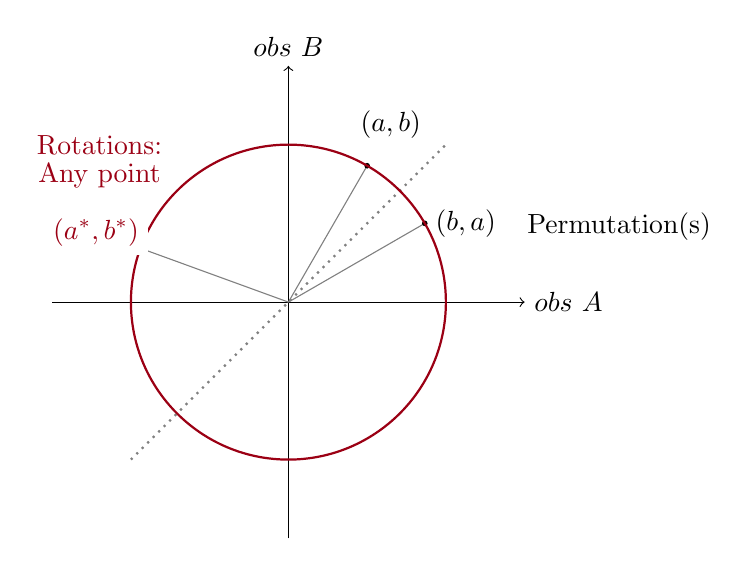
\begin{tikzpicture}[scale=2]
 \draw[->] (-1.5cm,0cm) -- (1.5cm,0cm) node[right,fill=white] {$obs\ A$};
        \draw[->] (0cm,-1.5cm) -- (0cm,1.5cm) node[above,fill=white] {$obs\ B$};
                                \draw[gray] (0cm,0cm) -- (60:1cm);
                \filldraw[black] (60:1cm) circle(0.4pt);
                                     \draw (60:1.3cm) node[fill=white] {$(a,b)$};
                    \pause
                \draw[gray, dotted, thick] (-1cm,-1cm) -- (1,1cm);                
               \pause

  %              \draw (60:0.6cm) node[fill=white] {$60^\circ$};
               \node at (2.1, .48) {Permutation(s)};
                \draw (30:1.3cm) node[below,fill=white] {$(b,a)$};


                \draw[gray] (0cm,0cm) -- (30:1cm);
                \filldraw[black] (30:1cm) circle(0.4pt);
   %             \draw (30:0.6cm) node[fill=white] {$30^\circ$};
\pause
  % draw the unit circle
        \draw[thick,color=redUnipd] (0cm,0cm) circle(1cm);

                \draw[gray] (0cm,0cm) -- (160:1cm);
                \filldraw[black] (160:1cm) circle(0.4pt);
%                \draw (160:0.6cm) node[fill=white] {$160^\circ$};
               \node at (-1.2,1) {\textcolor{redUnipd}{Rotations:}};
               \node at (-1.2,.8) {\textcolor{redUnipd}{Any point}};
                \draw (160:1.3cm) node[fill=white] {\textcolor{redUnipd}{$(a^*,b^*)$}};
      
\end{tikzpicture}
\end{center}
\end{frame}

%===================
\begin{frame}
\frametitle{Some properties}
\bi
\item Rotations of the orthogonalized residuals extends Permutations (i.e. orthogonal matrices with not all zeros and ones).
\item Both tests are approximated \\(and asymptotically exact and consistent),
\item When $\tilde{\mathbf{Y}}$ \emph{left-spherically distributed} (e.g. normal),  \\
$\tilde{\mathbf{Y}}  \stackrel{\mathrm{d}}{=} \tilde{\mathbb{O}}\tilde{\mathbf{Y}}$ i.e. exact test.
\medskip
\pause
\item Easy to generate from the joint distribution\\ i.e. dependence among tests is dealt.
\ei
\end{frame}
%%% ==========================
%\section{Multiplicity control}
%%% ==========================
\begin{frame}
\frametitle{... back to motivating example: ALL results}
\bi
\item Acute Lymphoblastic Leukemia data (Chiaretti et al., 2004)
\item $n =$ 128 patients,  $p =$ \textcolor{redUnipd}{12625 genes}
\item covariate of interest: {\tt group} (B or T-cell type patients)
\item \textcolor{redUnipd} {confounder(s): {\tt age} + {\tt sex} }
%\item differentially expressed genes between the two groups?
\pause
\item \textcolor{myblue}{\tt library(flip) \\ pvalues = flip(Y, X=$\sim$group, Z=$\sim$age+sex, \\ \ \ data=ALLdata, testType='rotation', perms=10000)}
\ei
\pause
\bb{Application to Multiplicity control:}
\bi
\item Familywise Error Rate:\\ parametric \& Holm vs permutation \& min-p
\pause
\item simultaneous CI for number of rejected hypos:
\\ parametric \& Simes vs permutation \& Meinshausen
\ei
\eb

\end{frame}
%%% ==========================
%%===============
%\begin{frame}
%\frametitle{Bonferroni vs min-p} 
%%\frametitle{Rotation null distribution of P-values}

%\begin{columns}

% \column{.45\textwidth} 

%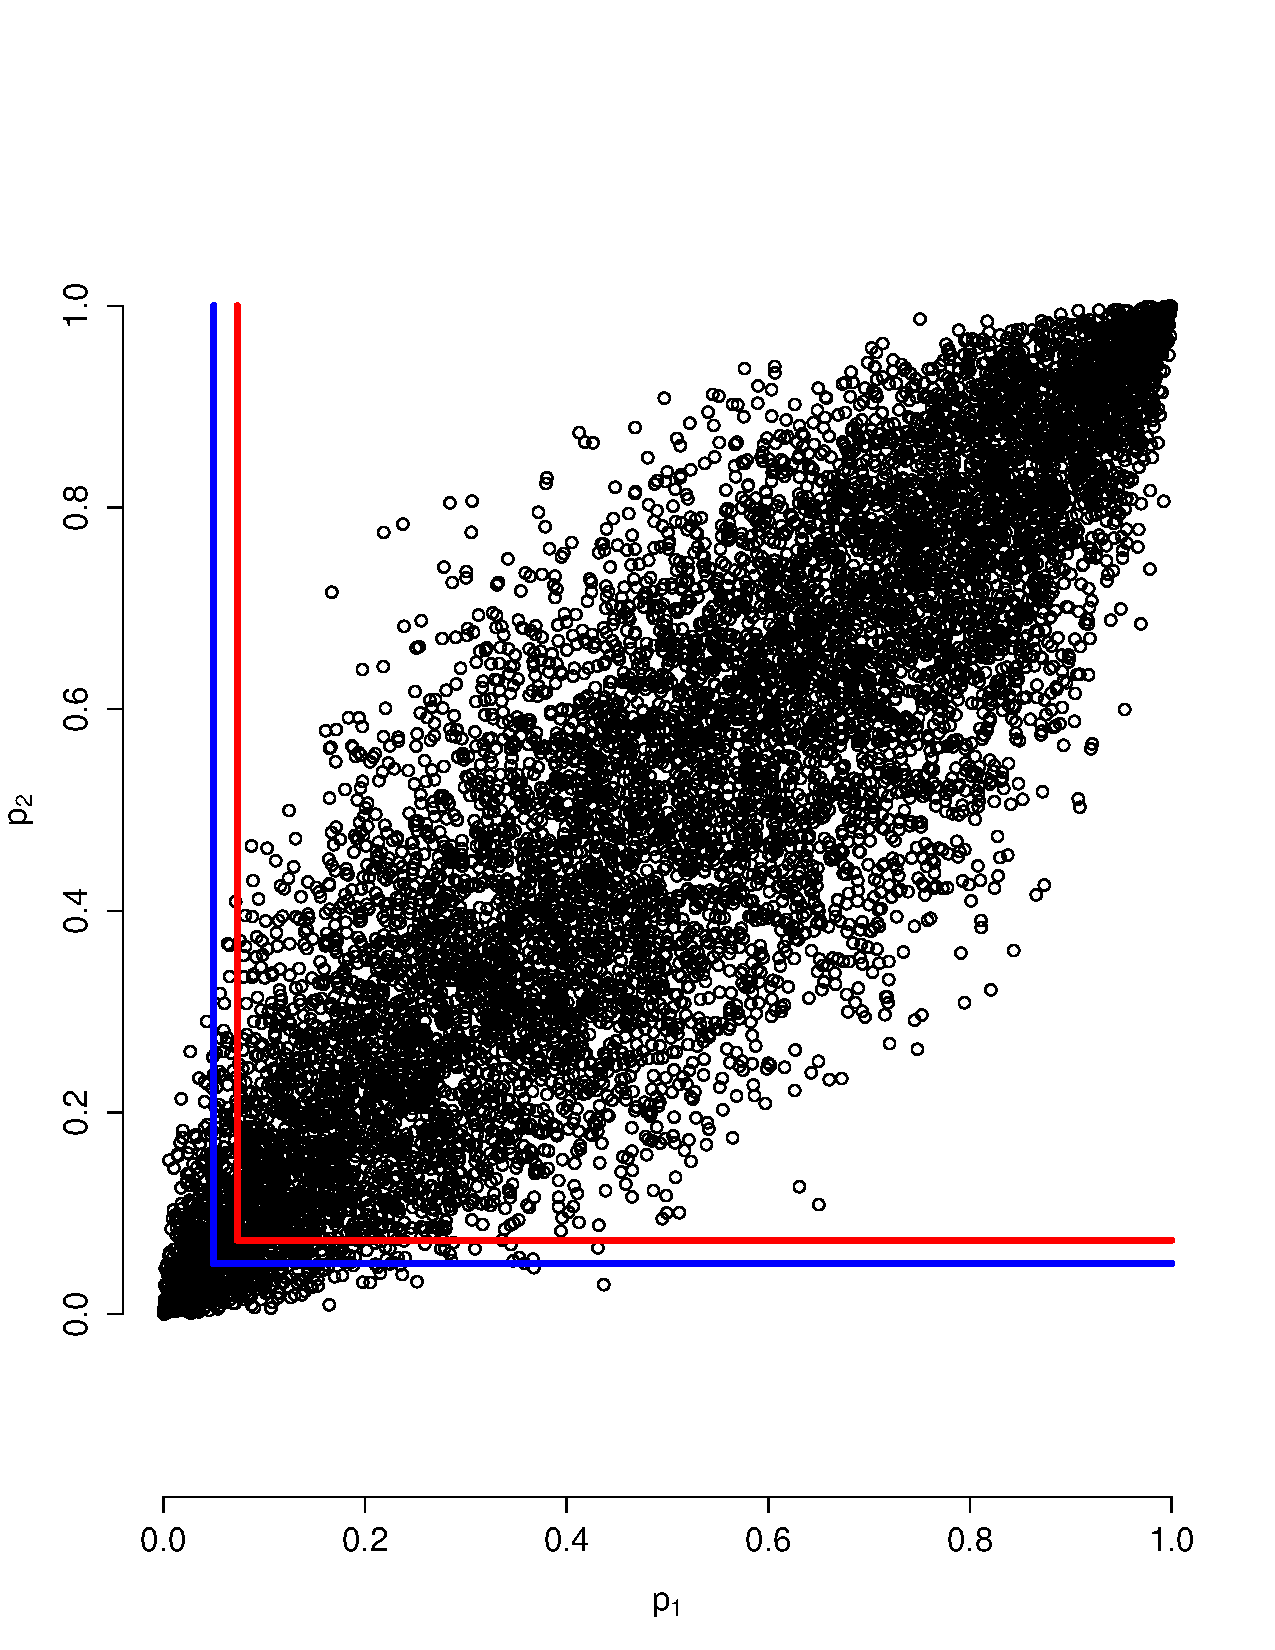
\includegraphics[scale=.28]{figures_perm_covariates/bonferroni}

% \column{.55\textwidth} 


%\bi

%\item Hypothesis:
%\[
%H: H_1 \cap H_2
%\]

%\item \textcolor{red}{min-P} test:
%\[
%\displaystyle \Pr_H\Big\{\min(p_1,p_2) < \textcolor{red}{c}\Big\} \leq \alpha
%\]


%\item \textcolor{blue}{Bonferroni} inequality:\\

%\[\textcolor{blue}{c=\alpha/2}\]

%\ei

%\end{columns}

%\end{frame}

%%% ==========================

%%% ==========================

\begin{frame}[fragile]
\frametitle{Familywise Error Rate (Holm vs min-p)}
%\begin{center}
\includegraphics[scale=.8]{figures_perm_covariates/compareRaw.pdf}\includegraphics[scale=.8]{figures_perm_covariates/compareAdj.pdf}
%\end{center}
\end{frame}

\begin{frame}[fragile]
\frametitle{Familywise Error Rate (Holm vs min-p)}
\begin{center}
\includegraphics[scale=1]{figures_perm_covariates/compareAdj10.pdf}
\end{center}

\end{frame}
\begin{frame}[fragile]
\frametitle{Familywise Error Rate (Holm vs min-p)}
\textcolor{myblue}{\tt res=flip.adjust(pvalues,'maxT')}
\includegraphics[scale=.45]{figures_perm_covariates/compareFWER2}

\end{frame}
%%% ==========================

\begin{frame}
\frametitle{Simes vs Meinshausen}
\textcolor{myblue}{\tt library(cherry);  curveMeinshausen(pvalues) }\\
\bigskip

\begin{columns}
 \column{.47\textwidth} 
\# of false rejections\\ (lower bound .95) 


\includegraphics[scale=.25]{figures_perm_covariates/ALL_numbers2}

 \column{.47\textwidth} 
Prop. of false rejections\\ (lower bound .95)

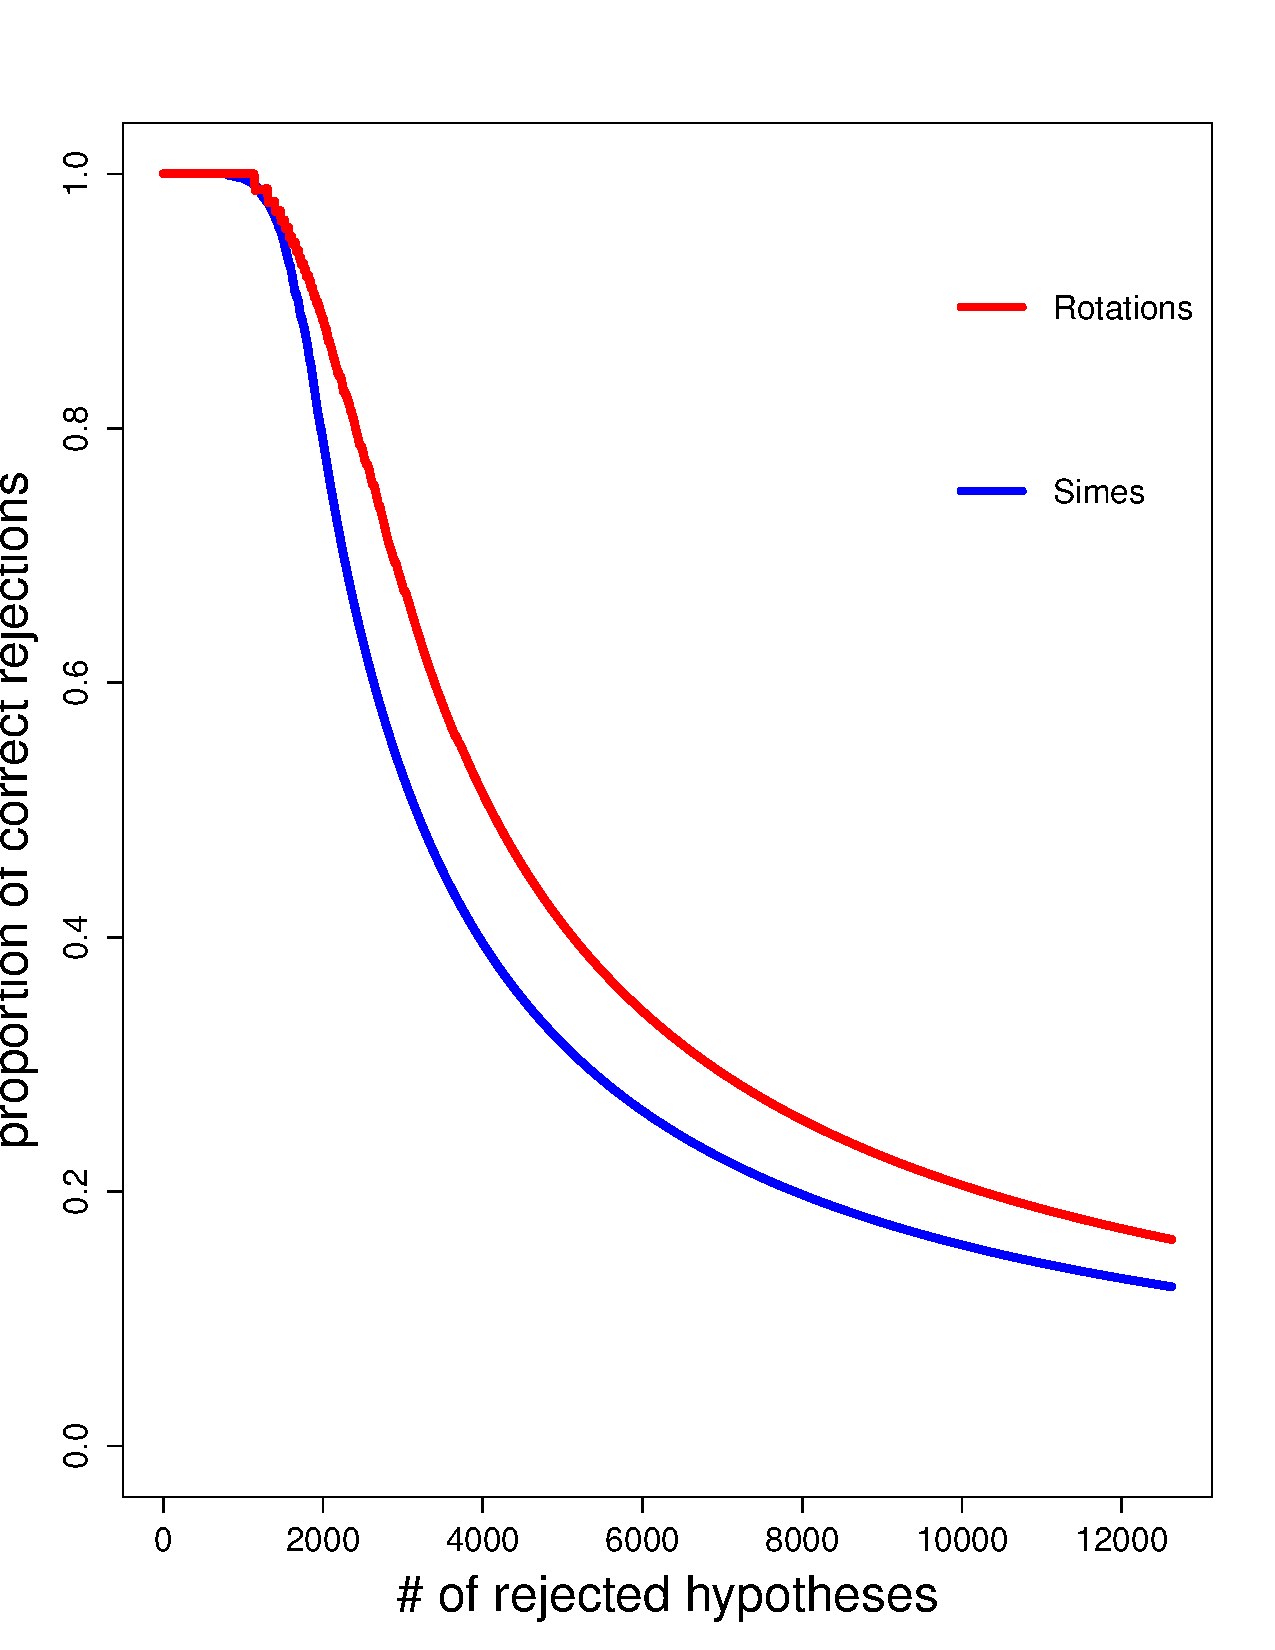
\includegraphics[scale=.25]{figures_perm_covariates/ALL_proportions}


\end{columns}



\end{frame}
%%% ==========================
\begin{frame}
\frametitle{Take-home message}

\bi
\item Permutations and Rotations \\
- easily deal with dependence, even when $p>>n$,\\
- more powerful multiplicity control\\
\pause
\item Adjusting for confounders
\pause
\bi
\item[]\textcolor{myblue}{discrete:} permutations within strata provide exact tests\\
\pause
$\ \ \ \ $ and require less assumptions on data
\pause
\item[] \textcolor{myblue}{continuous:} use orthogonal residuals (with permutations or rotations):
\bi 
\item[-] $2^{nd}-moment$ exact (i.e. approximated test, asymptotically exact)
\item[-] Exact for multivariate normal (i.e. left-spherical + independence)
\ei
\ei

\item simple algorithm even for high dimensional data
\item \textcolor{redUnipd}{R packages} {\tt 'flip'} and {\tt 'cherry'}
\ei

\end{frame}
%%%% ==========================

\end{document}
